% =====================================================================
%  Seance 6 -- E. Evaluation de l'UE, quiz final, cloture (29--33)
% =====================================================================
\section{Évaluation de l'UE et clôture}

\begin{frame}{Évaluation de l'UE EPD-GIT-5534}
\begin{center}
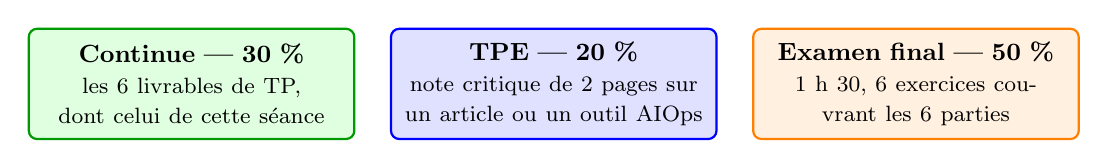
\begin{tikzpicture}[font=\small]
\node[draw=green!60!black, fill=green!12, rounded corners=3pt, thick,
      minimum height=14mm, text width=3.9cm, align=center] at (0,0)
  {\textbf{Continue --- 30 \%}\\ \normalfont\footnotesize les 6 livrables de
   TP, dont celui de cette séance};
\node[draw=blue, fill=blue!12, rounded corners=3pt, thick,
      minimum height=14mm, text width=3.9cm, align=center] at (4.6,0)
  {\textbf{TPE --- 20 \%}\\ \normalfont\footnotesize note critique de 2
   pages sur un article ou un outil AIOps};
\node[draw=orange, fill=orange!12, rounded corners=3pt, thick,
      minimum height=14mm, text width=3.9cm, align=center] at (9.2,0)
  {\textbf{Examen final --- 50 \%}\\ \normalfont\footnotesize 1 h 30,
   6 exercices couvrant les 6 parties};
\end{tikzpicture}
\end{center}
\vspace{2mm}
\begin{columns}[t]
\begin{column}{0.48\textwidth}
\begin{ebox}[TPE : ce qui est attendu]
Deux pages : un article ou un outil AIOps réel (par ex. une lecture sur
l'isolation forest appliquée aux métriques, ou un outil de monitoring),
résumé en 10 lignes + \textbf{votre} critique : que vaut la méthode sur des
données comme NOSYS ?
\end{ebox}
\end{column}
\begin{column}{0.48\textwidth}
\begin{kbox}[Examen final : les 6 exercices]
Un exercice par partie du syllabus : profil des données, préparation,
classification sur classe rare, séries temporelles, logs et sécurité,
industrialisation. Le quiz blanc du B4 en est le miroir exact.
\end{kbox}
\end{column}
\end{columns}
\end{frame}

\begin{frame}{Quiz final de clôture --- 6 QCM sur l'ensemble de l'UE (1/2)}
\begin{qbox}[Questions 1 à 3]
\begin{enumerate}
\item Séance 1--2 --- La première chose à faire devant une valeur
impossible (CPU à 350 \%) est :\\
(a) supprimer la ligne \quad (b) la convertir en manquant avec la borne
physique documentée \quad (c) la garder telle quelle
\item Séance 2 --- Le jeu supervisé contient 120 positives sur 34 560
fenêtres, soit :\\
(a) 3,5 \% \quad (b) 0,35 \% \quad (c) 12 \%
\item Séance 3 --- Sur une classe aussi rare, la métrique à regarder
d'abord est :\\
(a) l'exactitude (accuracy) \quad (b) le couple précision/rappel \quad
(c) le R²
\end{enumerate}
\end{qbox}
\vspace{1mm}
\begin{solbox}[Réponses]
\textbf{1 : b} \quad \textbf{2 : b} \quad \textbf{3 : b} --- l'accuracy
vaut déjà 99,65 \% en prédisant tout « pas d'incident ».
\end{solbox}
\end{frame}

\begin{frame}{Quiz final de clôture --- 6 QCM sur l'ensemble de l'UE (2/2)}
\begin{qbox}[Questions 4 à 6]
\begin{enumerate}
\item Séance 4 --- La validation d'un modèle de prédiction de panne doit
être :\\
(a) croisée aléatoire \quad (b) temporelle, le test strictement après le
train \quad (c) faite sur le train
\item Séance 5 --- La brute force du 5/10 sur \file{bdd-principal} se
détecte par :\\
(a) une hausse du CPU \quad (b) une séquence d'échecs d'authentification
concentrés dans le temps ($\approx$ 125) \quad (c) une baisse de latence
\item Séance 6 --- Sur les tranches de test sans incident, on surveille :\\
(a) l'AUC \quad (b) la distribution des scores et le taux d'alertes \quad
(c) rien
\end{enumerate}
\end{qbox}
\vspace{1mm}
\begin{solbox}[Réponses]
\textbf{4 : b} --- sinon fuite : le modèle aurait « vu » l'avenir \quad
\textbf{5 : b} \quad \textbf{6 : b}
\end{solbox}
\end{frame}

\begin{frame}{Les 6 messages de l'UE}
\begin{kbox}[Si vous ne retenez que six choses]
\begin{enumerate}
\item \textbf{Les données d'infrastructure ont des défauts systématiques} ---
audit avant réparation, granularité et horloges d'abord.
\item \textbf{L'étiquette est le cœur du projet} : « incident $\le$ 30 min »
regardant le futur, sans fuite --- 80 \% des échecs sont là.
\item \textbf{La classe rare impose ses métriques} : précision/rappel et
AUC, jamais l'accuracy.
\item \textbf{Le temps est une contrainte, pas un détail} : split temporel
strict, validation qui respecte la chronologie.
\item \textbf{Les logs complètent les métriques} : l'attaque du 5/10 était
invisible dans les métriques, criante dans les logs.
\item \textbf{Un modèle sans monitoring n'est pas un système} : registre,
latence mesurée, dérive surveillée, rollback écrit.
\end{enumerate}
\end{kbox}
\end{frame}

\begin{frame}{Et après ? --- merci, et la suite du parcours}
\footnotesize%
\begin{columns}[t]
\begin{column}{0.52\textwidth}
\begin{kbox}[Pour continuer seul(e)]
\begin{itemize}
\item \textbf{Deep learning appliqué aux séries temporelles} : réseaux
récurrents, puis les transformers pour la prédiction de charge.
\item \textbf{MLOps avancé} : CI/CD de modèles, déploiement canari,
détection de dérive statistique en continu.
\item \textbf{Certifications cloud} : les services de monitoring des grands
fournisseurs appliquent mot pour mot les concepts de cette UE.
\end{itemize}
\end{kbox}
\end{column}
\begin{column}{0.44\textwidth}
\begin{ebox}[Votre dossier de fin d'UE]
\begin{itemize}
\item \file{nosys\_features.csv} et son dictionnaire.
\item Le pipeline sauvegardé (\file{nosys\_pipeline.joblib}).
\item La fiche MLOps du B3.
\item La note critique TPE.
\end{itemize}
\end{ebox}
\begin{center}\small
Merci pour votre travail sur les six séances ---\\
le prochain système que vous monitorerez vous dira merci aussi.
\end{center}
\end{column}
\end{columns}
\end{frame}
